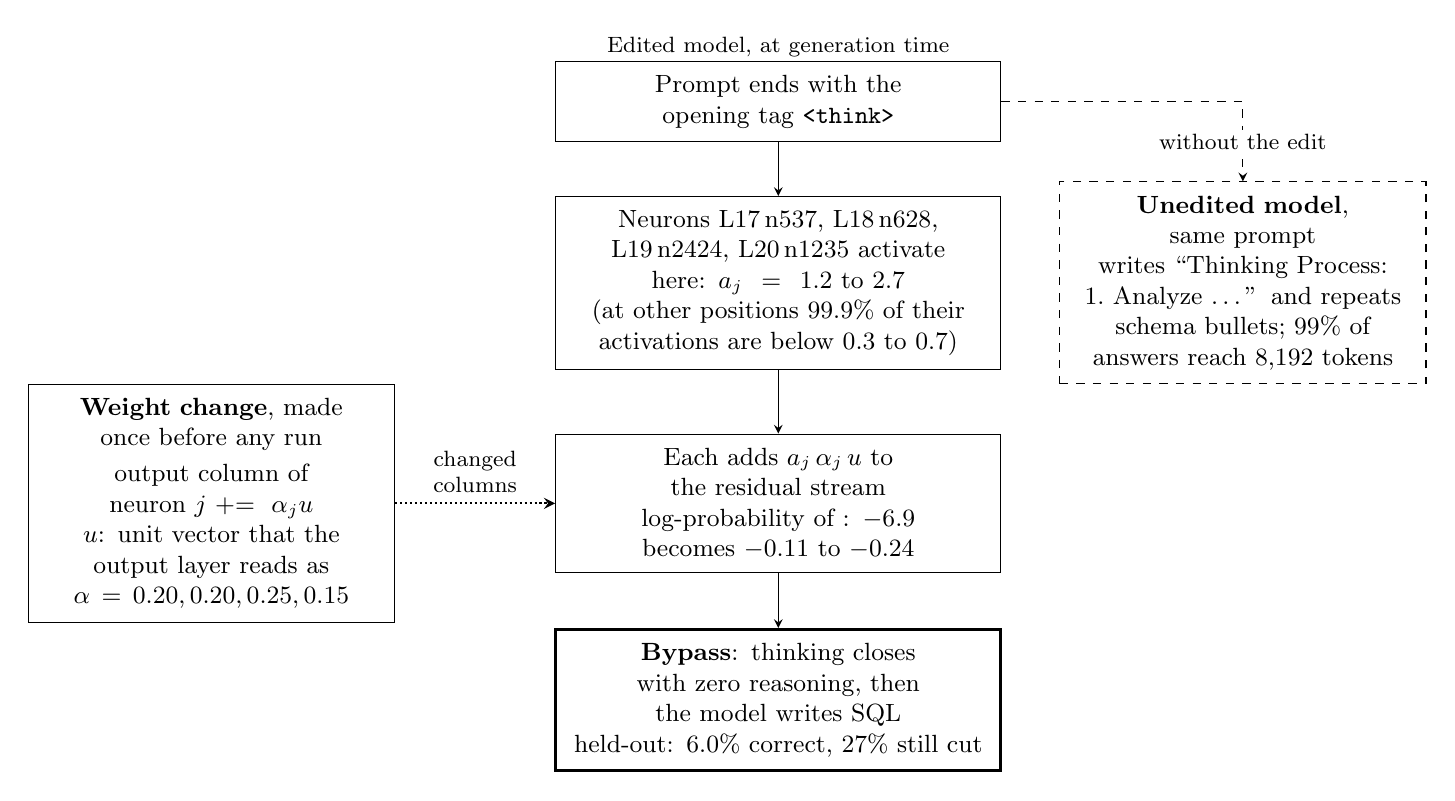
\begin{tikzpicture}[font=\small, box/.style={draw, align=center, execute at begin node={\hyphenpenalty=10000 \exhyphenpenalty=10000}, inner sep=5pt, text width=#1}, box/.default=5.3cm, lab/.style={font=\footnotesize, fill=white, inner sep=1.5pt, align=center}, >=stealth]
\node[box] (T) at (5.9,0) {Prompt ends with the opening tag \texttt{<think>}};
\node[box] (N) at (5.9,-2.3) {Neurons L17\,n537, L18\,n628, L19\,n2424, L20\,n1235 activate here: $a_j = 1.2$ to $2.7$\\(at other positions 99.9\% of their activations are below 0.3 to 0.7)};
\node[box] (R) at (5.9,-5.1) {Each adds $a_j\,\alpha_j\,u$ to the residual stream\\log-probability of \think{}: $-6.9$ becomes $-0.11$ to $-0.24$};
\node[box, very thick] (O) at (5.9,-7.6) {\textbf{Bypass}: thinking closes with zero reasoning, then the model writes SQL\\held-out: 6.0\% correct, 27\% still cut};
\node[box=4.3cm] (W) at (-1.3,-5.1) {\textbf{Weight change}, made once before any run\\[2pt]output column of neuron $j$ $\mathrel{+}=\alpha_j u$\\$u$: unit vector that the output layer reads as \think{}\\$\alpha = 0.20, 0.20, 0.25, 0.15$};
\node[box=4.3cm, dashed] (L) at (11.8,-2.3) {\textbf{Unedited model}, same prompt\\writes ``Thinking Process: 1.\ Analyze \ldots'' and repeats schema bullets; 99\% of answers reach 8,192 tokens};
\draw[->] (T) -- (N); \draw[->] (N) -- (R); \draw[->] (R) -- (O);
\draw[->, densely dotted, thick] (W.east) -- node[lab, above=2pt] {changed\\columns} (R.west);
\draw[->, dashed] (T.east) -| node[lab, pos=0.75] {without the edit} (L.north);
\node[font=\footnotesize, anchor=south] at (5.9,0.45) {Edited model, at generation time};
\end{tikzpicture}
